\documentclass[12pt,a4paper,twoside]{scrartcl}
\usepackage[english,ngerman]{babel}
\usepackage[T1]{fontenc}
\usepackage{lmodern}
\usepackage[utf8]{inputenc}
\usepackage[tmargin=22mm,bmargin=22mm,lmargin=20mm,rmargin=20mm]{geometry}
\usepackage{latexsym,amsmath,amssymb,mathtools,textcomp}
\usepackage{parskip}
\usepackage{amsthm}
\usepackage{bbm}
\usepackage{mathtools}
\usepackage{indentfirst}
\usepackage{setspace}
\usepackage{csquotes}
\begingroup
\makeatletter
\@for\theoremstyle:=definition,remark,plain\do{%
  \expandafter\g@addto@macro\csname th@\theoremstyle\endcsname{%
    \addtolength\thm@preskip\parskip
  }%
}
\endgroup

\newtheorem{theorem}{Theorem}[section]
\newtheorem{definition}[theorem]{Definition}
\newtheorem{lemma}[theorem]{Lemma}

\numberwithin{equation}{section}
\DeclareOldFontCommand{\bf}{\normalfont\bfseries}{\mathbf}

\usepackage{graphicx}
\graphicspath{{images/}}
\usepackage{array,multirow}
\usepackage{enumitem}
\setlist[enumerate]{topsep=0pt}
\setlist[itemize]{topsep=0pt}
\setlist[description]{font=\normalfont,topsep=0pt}


\usepackage{float}
\usepackage{tikz}
\usetikzlibrary{calc}
\usepackage{fancyhdr}
\fancypagestyle{plain}{
  \setlength\footskip{32pt}
  \fancyhead{}
  \fancyfoot{}
  \fancyfoot[LE,RO]{\normalsize\thepage}
  \renewcommand{\headrulewidth}{0pt}
  \renewcommand{\footrulewidth}{0pt}
}

\usepackage{ctable}
\fancypagestyle{normal}{
  \setlength{\headheight}{20pt}
  \setlength\footskip{32pt}
  \fancyhead{}
  \fancyhead[LE]{\normalsize\textsc{\nouppercase{\leftmark}}}
  \fancyhead[RO]{\normalsize\textsc{\nouppercase{\rightmark}}}
  \fancyfoot{}
  \fancyfoot[LE,RO]{\normalsize\thepage}
  \renewcommand{\headrulewidth}{0.4pt}
  \renewcommand{\footrulewidth}{0pt}
}

\usepackage{color}
\usepackage[pagebackref]{hyperref}
\usepackage[all]{hypcap}
\usepackage{cleveref}
\usepackage[font=small,belowskip=6pt]{subcaption}
\usepackage[section]{placeins}

\usepackage[titletoc,toc,title,page]{appendix}
\usepackage{pdfpages}
\usepackage[export]{adjustbox}

\usepackage{pgfplots}
\usepackage{tikz}
\usepackage{lmodern}
\usepackage{multirow}
\usepackage{makecell}
\usepackage{boldline}
\usepackage{array}
\usepackage{caption}
\usepackage{varwidth}
\usepackage{threeparttablex}
\usepackage{rotating}


\hypersetup{
  pdftitle={Automatische Auswahl von maschinellen Lernverfahren für kausale Inferenz},
  pdfauthor={Atanas Dimitrov}, 
  pdfsubject={causal inference,synth validation, machine learning, gradient boosting, lasso, causal forest}
  colorlinks=true,
  pdfborder={0 0 0},
  bookmarksopen=true,
  bookmarksopenlevel=1,
  bookmarksnumbered=true,
  linkcolor=blue!60!black,
  % linkcolor=black,
  citecolor=blue!60!black,
  urlcolor=blue!60!black,
  filecolor=green!60!black,
  pdfpagemode=UseNone,
  unicode=true,
}
\renewcommand{\appendixpagename}{\appendixname} 
\renewcommand{\appendixtocname}{\appendixname}

\renewcommand{\baselinestretch}{1.2} 
\renewcommand*{\backreflastsep}{, }
\renewcommand*{\backreftwosep}{, }
\renewcommand*{\backref}[1]{}
\renewcommand*{\backrefalt}[4]{%
  \ifcase #1 %
  Keine Zitierungen.
  \or
  (Seite #2).%
  \else
  (Seiten #2).%
  \fi%
}
\usepackage{import}

\newcommand{\reflst}[1]{\hyperref[#1]{Listing~\ref*{#1}}}
\newcommand{\refthm}[1]{\hyperref[#1]{Theorem~\ref*{#1}}}
\newcommand{\refdef}[1]{\hyperref[#1]{Definition~\ref*{#1}}}

\newcommand{\reffig}[1]{\hyperref[#1]{Figure \ref*{#1}}}
\newcommand{\refsec}[1]{\hyperref[#1]{Section \ref*{#1}}}
\newcommand{\reftab}[1]{\hyperref[#1]{Table \ref*{#1}}}
\newcommand{\refapp}[1]{\hyperref[#1]{Appendix \ref*{#1}}}

\renewcommand*{\refeq}[1]{\hyperref[#1]{Equation \ref*{#1}}}

\renewcommand\theadalign{bc}
\renewcommand\theadfont{\bfseries}
\renewcommand\theadgape{\Gape[4pt]}
\renewcommand\cellgape{\Gape[4pt]}

\newcolumntype{L}[1]{>{\raggedright\let\newline\\\arraybackslash\hspace{0pt}}m{#1}}
\newcolumntype{C}[1]{>{\centering\let\newline\\\arraybackslash\hspace{0pt}}m{#1}}
\newcolumntype{R}[1]{>{\raggedleft\let\newline\\\arraybackslash\hspace{0pt}}m{#1}}



\newcounter{mypagecount}% create a new counter
\setcounter{mypagecount}{0}% set it to something just in case
\newenvironment{interlude}{% create a new environment for the unnumbered section(s)
  \clearpage
  \setcounter{mypagecount}{\value{page}}% use the new counter we created to hold the page count at the start of the unnumbered section
  \thispagestyle{empty}% we want this page to be empty (adjust to use a modified page style)
  \pagestyle{empty}% use the same style for subsequent pages in the unnumbered section
}{%
  \clearpage
  \setcounter{page}{\value{mypagecount}}% restore the incremented value to the official tally of pages so the page numbering continues correctly
}

% Package for inserting pseudo codes in the document.
\usepackage[ruled,vlined,linesnumbered,norelsize]{algorithm2e}
\DontPrintSemicolon
\def\NlSty#1{\textnormal{\fontsize{8}{10}\selectfont{}#1}}
\SetKwSty{texttt}
\SetCommentSty{emph}
\def\listalgorithmcfname{List of Algorithms}
\def\algorithmautorefname{Algorithm}
\let\chapter=\section % resolve a problem with algorithm2


\begin{document}
\boldmath
\nonfrenchspacing

\pagestyle{empty}
\pagenumbering{alph}


\setlength{\parindent}{4em}
\setlength{\parskip}{1em}

% title page
\begin{titlepage}

  \begin{center}\large

    {\flushleft
\includegraphics[height=17mm, width=45mm]{kit_logo_en.pdf} \hfill}
    
\includegraphics[height=15mm, width=45mm]{group_logo.pdf}\quad\null

    \vspace*{1cm}
    {\Large Bachelorarbeit}\\
    \noindent\hfil\rule{0.4\textwidth}{.4pt}\hfil
    \vspace*{1cm}

    {\bf\huge Automatische Auswahl von maschinellen Lernverfahren für kausale Inferenz\par}
    \vspace*{5mm}

    von\\
    \vspace*{3mm}
    {\huge{Atanas Dimitrov}}

    \vspace*{10mm}
    Pervasive Computing Systems / TECO\\
    Institut für Telematik\\
	Fakultät für Informatik\\
   
    \vspace*{15mm}

   	Abgabadatum: 02.09.2019 %TODO
    \vspace*{10mm}


    \begin{tabular}{p{8cm}l}
     Verantwortlicher Betreuer: &Prof. Dr. Michael Beigl\\
     Betreuerin: &Ployplearn Ravivanpong\\  
    \end{tabular}

    \vspace*{8mm}

  \end{center}

\end{titlepage}

\selectlanguage{ngerman}

\centerline{\bf\large Erklärung}

\vspace*{12mm}

{\setstretch{1.5}\large Hiermit erkläre ich, dass ich die vorliegende Bachelorarbeit selbstständig verfasst und keine anderen als die angegebenen Hilfsmittel und Quellen benutzt habe, die wörtlich oder inhaltlich übernommenen Stellen als solche kenntlich gemacht und weiterhin die Richtlinien des KIT zur Sicherung guter wissenschaftlicher Praxis beachtet habe.\par}

\vfill
\noindent
{\large Karlsruhe, 02.09.2019}
\hrule


\vspace*{5cm}

\clearpage

%%%%%%%%%%%%%%%%%%%%%%%%%%%%%%%%%%%%%%%%%%%%%%%%%%%%%%%%%%%%%%%%%%%%%% 

\vspace*{0pt}\vfill

\selectlanguage{ngerman}

\begin{abstract}
  \centerline{\bf Abstract}
  \vspace*{1cm}
 Diese Bachelorarbeit beschäftigt sich mit dem Vergleich von Methoden für kausale Inferenz und mit der automatischen Auswahl von dem besten von denen abhängig von dem vorhandenen Datensatz. Dazu benutzen und erweitern wir Synth-Validation - ein Verfahren, mit dem von den echten Daten synthetische Daten mit einem gewünschtem durchschnittlichen Behandlungseffekt erstellt und dann ausgewertet werden. Dabei haben die Datensätze, auf denen wir unsere Experimente durchführen, unterschiedliche Natur - echten Rohdaten mit größeren oder kleineren Zahl von Kovariaten, von Rohdaten synthetisch generierten Daten und zufällig generierten Daten. Die kausale Inferenz Verfahren, von denen Synth-Validation auswählt, benutzen ausschließlich Algorithmen aus dem maschinellem Lernen. Es wird die Fähigkeit von Synth-Validation gemessen, den Verfahren zu wählen, der die nächste Schätzung von dem durchschnittlichen Behandlungseffekt hat. Das wird unter unterschiedlichen Konstellationen unterstellt - nach der Art der Daten, nach der Anzahl der Elementen in der Stichprobe usw.          
\end{abstract}

\vfill\vfill\vfill
\clearpage

%%%%%%%%%%%%%%%%%%%%%%%%%%%%%%%%%%%%%%%%%%%%%%%%%%%%%%%%%%%%%%%%%%%%%% 
\selectlanguage{ngerman}
\pagestyle{plain}
\pagenumbering{roman}

% markiere sections im Seitenkopf links und subsections rechts
\renewcommand\sectionmark[1]{\markboth{\thesection\quad\MakeUppercase{#1}}{\thesection\quad\MakeUppercase{#1}}}
\renewcommand\subsectionmark[1]{\markright{\thesubsection\quad\MakeUppercase{#1}}}

\tableofcontents
\clearpage
%%%%%%%%%%%%%%%%%%%%%%%%%%%%%%%%%%%%%%%%%%%%%%%%%%%%%%%%%%%%%%%%%%%%%% 
\listoffigures
\clearpage

\pagestyle{normal}
\pagenumbering{arabic}

%main content starts here
\nocite{*} %TODO remove when all references ready 
\section{Einführung}\label{sec:einführung}
Um die Welt besser zu verstehen, haben die Menschen immer die Antwort auf der folgenden Frage gesucht: Was passiert, wenn eine bestimmte Tat oder Handlung durchgeführt wird? Manche Handlungen kann man als \enquote{einfach} qualifizieren und bei denen ist diese Antwort leicht zu erreichen. Wenn man einen Apfel nach oben wirft, fällt er wieder nach unten. Es kostet (fast) nichts, diese Tatsache zu prüfen. Fast jeder kann dieses Ergebnis vorhersagen, weil man irgendwann mal ein fallendes Objekt beobachtet hat, unabhängig davon, ob man weiß, warum die Objekte fallen. Handlungen können aber deutlich komplexer sein wie z.B. Einnahme einer neuen Steuerpolitik oder die medizinische Behandlung mit einem Medikamenten. Diese Handlungen sind schwerer durchzuführen, sind von mehreren Faktoren oder Naturgesetzen betroffen, sind \enquote{abhängiger}. Auf Basis früherer Erfahrung im Bereich können Experten Rahmen davon setzen, was passieren wird. Sicher kann man nur dann sein, wenn die Handlung durchführt ist und man beobachtet und bemesst, was passiert hat. Die letzte Schlussfolgerung gilt sowohl für die \enquote{einfacheren}, als auch für die \enquote{komplexeren} Handlungen. Also um eine sichere Kenntnis zu erschaffen, brauchen wir Erfahrung - in dem Fall mit dem Apfel entweder werfen wir den alleine oder beobachten wir jemanden, der das macht oder der das irgendwann mal gemacht hat. Bei den \enquote{komplexeren} Handlungen ist meistens die Antwort auf der Frage \enquote{Was?}  nicht ausreichend - man braucht \enquote{Wie viel?}. Das führt uns langsam zu dem Sachverhalt der kausalen Inferenz.      
  	\subsection{Kausale Inferenz}\label{subsec:kausalität}
  	Wenn wir über die Kausalität in ihrem wissenschaftlichen Sinn sprechen, muss es klar sein, dass \enquote{\textbf{\textit{A}} verursacht \textbf{\textit{B}}} nicht bedeutet, dass \textbf{\textit{A}} der Hauptgrund ist, warum \textbf{\textit{B}} passiert hat. Es bedeutet, dass \textbf{\textit{A}} den Unterschied oder die Differenz gemacht hat, die zu \textbf{\textit{B}} geführt haben. Es existieren möglicherweise noch weitere Gründe z.B. \textbf{\textit{C}} und \textbf{\textit{D}}, ohne deren Existenz und ohne deren verursachten Differenz \textbf{\textit{B}} nicht möglich war oder nicht den Wert halten würde, den es hält. \textbf{\textit{A}} soll man nicht als eine Zuschreibung von \textbf{\textit{B}} anschauen, sondern als einen Beitrag\cite{MacHum}.  Dabei sollen wir unter \textbf{kausale Inferenz} ähnlich wie bei der statistischen Inferenz den Prozess und die Methodiken zum Finden von Kenntnissen über die Kausalität von irgendeiner Handlung, insbesondere das Finden von der Differenz, die sie verursacht.\par
  	

\noindent	
Die kausale Inferenz hat aber ein fundamentales Problem. Wenn wir den Effekt von einer Handlung wissen wollen, führen wir diese Handlung aus und bemessen den Wert von irgendeine Variable, die uns interessiert. Der echte Effekt ist aber die Differenz zwischen dieser Variable bedingt, dass wir die Handlung durchgeführt haben und die gleiche Variable, bedingt, dass wir die Handlung nicht durchgeführt haben. Natürlich ist nur eine der beiden Optionen direkt beobachtbar. Formal kann man es so dargestellt: \par
  	
\begin{equation}
  TE = (Y|W = 1) - (Y|W = 0)
\end{equation}  	
  	
\noindent	  	
Hier bezeichnet \textbf{\textit{TE}} das Behandlungseffekt, \textbf{\textit{Y}} ist die beobachtete Variable und \textbf{\textit{W}} ist eine binäre Variable, die bezeichnet, ob die Handlung durchgeführt wurde oder nicht.\par

\noindent	  	
Obwohl wir den Behandlungseffekt von einer Handlung individuell nicht beobachten können, können wir schätzen, wie hoch durchschnittlich diesen Effekt ist, wenn wir die Handlung auf mehreren Objekten durchführen beziehungsweise auch auf mehreren nicht durchführen und die Differenz zwischen diesen beiden Ergebnissen als \textbf{durchschnittliches Behandlungseffekt} oder auf Englisch \textbf{average treatment effekt(ATE)} bezeichnen. Meistens können wir die Behandlung nicht auf allen (oder eigentlich auf der Hälfte von allen) Objekten durchführen, sondern müssen wir eine Stichprobe ziehen.  Formal stellen wir das so dar: \par

\begin{equation}\label{eq:1.2}
  \tau = E_Y[Y|W = 1] - E_Y[Y|W = 0]
\end{equation}

\noindent
In dieser Modelldarstellung sind $W$ und $Y$ Zufallsvariablen. $W$ ist binär, wo \textbf{1} für eine Behandlung und \textbf{0} für keine Behandlung steht. $Y$ ist die Zufallsvariable von einem gewünschten Wert nach der potenziellen Behandlung. $E_Y$ steht für den Erwartungswert von \textbf{Y}. Schon in dieser Darstellung treffen wir allen Problemen, die man sonst in der statistischen Inferenz trifft - damit unsere Schätzung über die Stichprobe näher zu der echten ATE der Gesamtpopulation liegt, müssen bestimmte Regeln eingehalten werden.\par

\noindent
Gleichung \ref{eq:1.2} ist immer noch kein gutes Model der Wirklichkeit, weil es oft der Fall ist, dass die Objekten, die wir behandeln, sich durch einigen Merkmalen unterscheiden. Diese andere Differenzen können Einfluss auf $Y$ sowohl bedingt $W$, als auch unbedingt $W$ haben und diese Tatsache soll in der Gleichung einbezogen werden:\par

\begin{equation}\label{eq:1.3}
  \tau = E_{Y,X}[Y|X,W = 1] - E_{Y,X}[Y|X,W = 0]
\end{equation}       	

\noindent 
$X$ ist eine Zufallsvariable für die so genannten \textbf{Kovariaten}. $X$ ist mehrdimensional und stellt den Zustand, in dem sich ein Objekt oder allgemeiner gesagt eine Welt befindet. Die Kovariaten sollen nicht, aber können einen Einfluss auf das Ergebnis $Y$ haben. Diejenigen mit Einfluss nennen wir \textbf{Confounders} oder \textbf{confounding Variablen}. Auf Deutsch kann man den Begriff am nächsten mit dem Wort Verwirrungsvariablen übersetzen. Die Existenz von Confounders erschwert unsere Aufgabe, den Effekt zu finden, den die Behandlung verursacht.\cite{vanderweele2013definition}. \par

\noindent
In der Tat können Confounders auch indirekten Einfluss auf die Behandlung haben. Beispiel: Sei $X$ das Alter sein, $W$ - ob man raucht oder nicht und $Y$ - eine Gesundheitsmaß. Es ist klar, dass das Alter an sich einen Effekt auf der Gesundheit hat. Die empirische Daten zeigen aber auch, dass das Rauchen unter älteren Menschen verbreiteter ist als unter jüngeren, d.h das Alter bewirkt sowohl das Rauchen, als auch die Gesundheit, die an sich vom Rauchen bewirkt wird. Diese Abhängigkeiten werden in Abbildung \ref{fig:confounder} veranschaulicht.\par   	
\begin{center}
  \vspace{6mm}
  \begin{figure}[h]
    \centering
    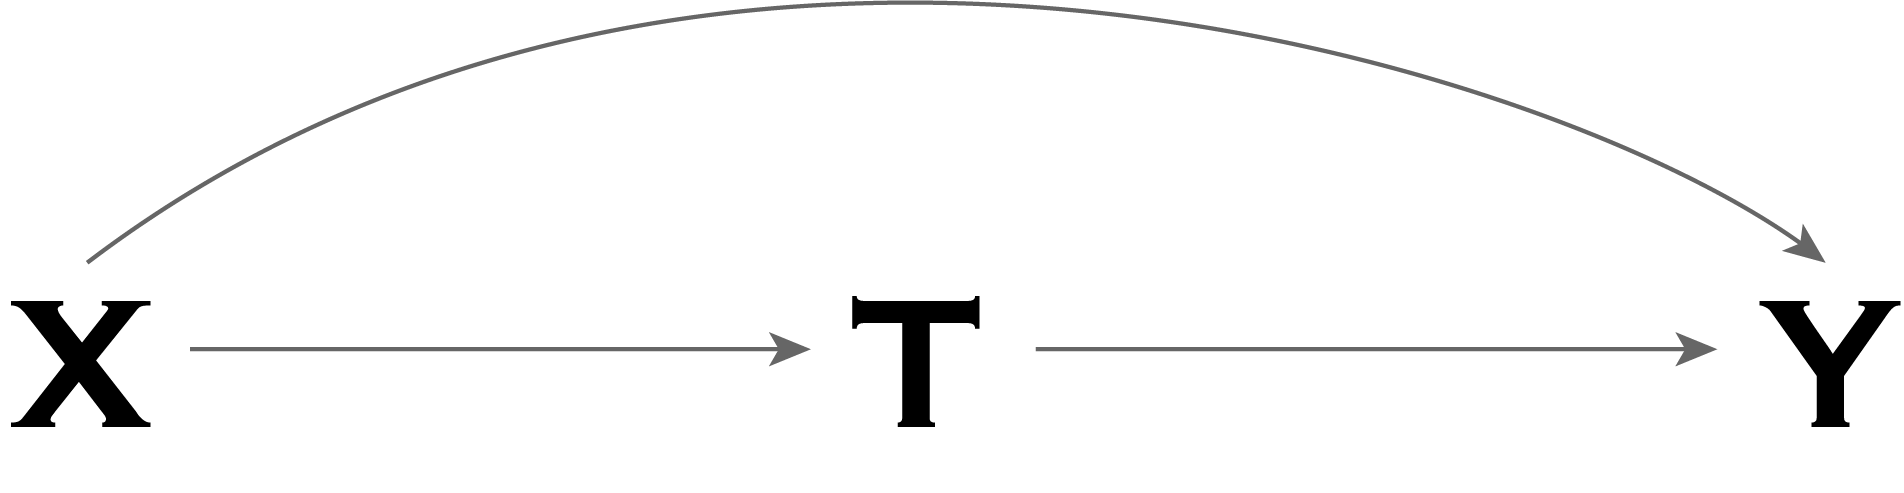
\includegraphics[height=0.4\textwidth, width=0.9\textwidth]{figures/confounder.png}
    \caption[Einfluss von Confounder auf Behandlung und Ergebnis]{Einfluss von Confounder auf Behandlung und Ergebnis. Hier ist $X$ der Confounder, $T$ - die Behandlung und $Y$ - das Ergebnis. Es wird gezeigt, dass das Ergebniss nicht nur von der Behandlung abhängt, sondern auch vom Confounder. Der Confouder hat auch eine Auswirkung auf die Behandlung.\cite{RebBar} }\label{fig:confounder}
  \end{figure}
\end{center}

\noindent
Wir schließen diesen Abschnitt mit der Gedanke von dem Philosophen David Lewis über die Kausalität, der sie folgendermaßen beschreibt: \enquote{etwas, was einen Unterschied verursacht und der Unterschied, den dieses etwas verursacht, soll der Unterschied  davon sein, was ohne dieses etwas passieren würde} \cite{lewis1974causation}.\par

\subsection{Motivation}\label{subsec:motivation}
Es ist wichtig zu wissen, was genau eine Handlung verursacht oder welche Differenz sie macht. Mit diesen Kenntnissen können wir besser die passenden Handlungen und deren genauen Maßen zum Erreichen unseres Ziels einschätzen und dann auswählen. Diese Behauptungen sind allgemeingültig und wir betrachten konkret drei Beispiele von unterschiedlichen Bereichen, wo das Kennen von dem durchschnittlichen Behandlungseffekt von großer Bedeutung ist.\par

\noindent
\textbf{Beispiel 1}\phantomsection\label{motivationBeispiel1} In der Pharmazie spielt die Kausalität eine besonders große Rolle. Wenn man einen Medikamenten entwickelt, soll man ganz genau wissen, welchen durchschnittlichen Effekt dieses Medikament auf unterschiedenen variablen körperlichen Werten hat - sowohl für wohltuende, als auch für schädliche Effekte. Hier ist das Nutzen, das die kausale Inferenz bringt, die Gesundheit der Menschen.\par

\noindent
\textbf{Beispiel 2}\phantomsection\label{motivationBeispiel2} Weitere Bedeutung hat die kausale Inferenz im Marketing und in der Bewertung von Werbungen. Eine Werbung kann eine Kette von unterschiedlichen Zielen haben, aber am Ende steht die Erhöhung von tatsächlichen Einkäufen von dem geworbenen Produkt oder Dienstleistung. Natürlich ist die Werbung nicht der einzige Treiber des Umsatzes. Also man muss nur den Effekt der Werbung einschätzen. Dann abhängig von diesem durchschnittlichen Effekt und dem Preis der Werbung stellt man fest, ob eine Werbung Nutzen bringt bzw. welche Werbung am nützlichsten ist.\par

\noindent
\textbf{Beispiel 3}\phantomsection\label{motivationBeispiel3} Die kausale Inferenz ist bedeutend für die Auswahl vom eigenen Verhalten sein. Zum Beispiel kann man den Einfluss vom regelmäßigen Rauchen von Rauschgift auf die mentalen Fähigkeiten untersuchen. Wenn man diesen durchschnittlichen Effekt kennt, sollte es wahrscheinlicher sein, dass man auf diese schlechte Sucht verzichtet oder am besten gar nicht damit anfängt. Diese deutliche wissenschaftliche Daten können durch den Gesetzgeber als Rechtfertigung für einen Verbot von diesem Stoff benutzt werden.\par
\subsection{Finden von ATE}\label{subsec:findenATE}
\noindent
\textit{Wir gehen davon aus, dass unser Problem schon klar definiert ist: Welchen durchschnittlichen Effekt(ATE) verursacht eine Behandlung? In diesem Abschnitt erläutern wir, wie man genau mit diesem Problem in den unterschiedlichen Situationen umgeht.}\par

\vspace{7mm}

Grundsätzlich muss man Gleichung \ref{eq:1.3} lösen, die wir zur Bequemlichkeit hier noch mal hinbringen.\par 

\begin{equation}\label{eq:1.4}
  \tau = E_{Y,X}[Y|X,W = 1] - E_{Y,X}[Y|X,W = 0]
\end{equation}  

\noindent
Dazu gibt es zwei Vorgehensweisen, die sich durch die Art von Datensammlung unterscheiden - Durchführung von einem Experimenten und Durchführung von einer Beobachtungsstudie. Die Daten aus den unterschiedlichen Studien wertet man dann anders aus.\par

\subsubsection{Experimentdurchführung}\label{subsubsec:experimentdurchführung}

Es gilt, dass der durch Daten von Experimenten geschätzte Behandlungseffekt weniger Bias hat und deswegen näher zu dem echten durchschnittlichen Effekt der Population  liegt. Der Grund dafür ist, dass die Objekten für die beiden Gruppen zufällig ausgewählt sind und somit wie die Population verteilt sind. Man soll immer diese Art von Datensammlung für kausale Inferenz wählen, wenn sie möglich ist. Von den in Abschnitt \ref{subsec:motivation} erwähnten Beispielen ist es bei Beispielen 1 und 2 möglich. 

\clearpage
\noindent
Das Experiment läuft folgendermaßen durch: zwei Gruppen von Objekten  werden gebildet. Die erste Gruppe heißt Behandlungsgruppe und die zweite  - Kontrollgruppe. Die Objekten von der ersten Gruppe werden mit irgendetwas z.B. einem Medikamenten behandelt, diese in der zweite jedoch nicht. Alle anderen Konditionen, auf die die Objekten in der Kontrollgruppe unterlegt sind, sollen sich nicht unterscheiden. Natürlich bleiben aber die einzelnen Objekten unterschiedlich, was zu unterschiedlichen Ergebnissen bei den individuell gemessenen Werten  führt. Uns interessiert aber der durchschnittliche Wert von jeder Gruppe. Deswegen muss sichergestellt werden, dass die Objekte in jeder Gruppe gleichmäßig verteilt sind. Es gibt unterschiedliche Strategien das zu erreichen. Eine der besten, wenn sie richtig durchgeführt wird, ist die zufällige Auswahl von Objekten aus der Population für jede Gruppe. Am Ende wird für jedes Objekt der Wert von Bedeutung gemessen. Die Mittelwerten von diesen Werten werden für jede Gruppe berechnet und die Differenz dazwischen ist der erwartete durchschnittliche Behandlungseffekt.  
\par

\noindent
Man kann auch Daten von den beiden Gruppen benutzen, um signifikanten Aussagen über den durchschnittlichen Behandlungseffekt mit einer bestimmten Konfidenz zu treffen. Dazu führt man meistens einen statistischen $t$-test durch. Man erstellt erstmal eine Nullhypothese und prüft, ob diese abzulehnen ist. Dafür berechnet man erstmal die Teststatistik $t$, die hier dargestellt ist:\par

\begin{equation}
  t = \sqrt{\frac{n_0n_1}{n_0+n_1}}\frac{\overline{Y_1}-\overline{Y_0}-\omega}{s}
\end{equation} 

\begin{equation}
  s = \sqrt{\frac{(n_0-1)s_0^2+(n_1-1)s_1^2}{n_0+n_1-2}}
\end{equation} 

\noindent
$n_0$ und $n_1$ sind die Anzahl von Objekten in den beiden Gruppen, $\overline{Y_1}$ und $\overline{Y_0}$ - die Mittelwerte von den Ergebnissen, $s_0^2$ und $s_1^2$ - die Varianzen, $s$ - die gewichtete Abweichung, $\omega$ - den Wert von dem durchschnittlichen Behandlungseffekt, den man für die Nullhypothese genommen hat. Dann abhängig davon, was man testen will und mit welcher Konfidenz die Behauptung gültig sein soll, vergleicht man den Wert von $t$ mit dem Wert von einem Quantil von der studentischen $t$-Verteilung. Am Ende hat man eine Behauptung, die mit irgendeiner Signifikanz wahr ist.\cite{ttest}    
\par    

\subsubsection{Beobachtungsstudiedurchführung}\label{subsubsec:beobachtungsstudietedurchführung}

Wir wiederholen noch mal, dass man lieber ein Experiment anstatt einer Beobachtungsstudie durchführen muss, um die Daten zu sammeln, wenn es möglich ist. Und natürlich ist es wegen unterschiedlichen Gründen nicht immer so.\par 

\noindent
Grundsätzlich kann ein Experiment viel mehr als eine Beobachtungsstudie kosten, weil man die Objekten (die Leuten) in experimentellen Bedingungen haben möchte. Man hat (höhere) Kosten für:\par

\begin{itemize}
  \item Vergütung der Leute
  \item die Behandlung
  \item Mitarbeiter, die das Experiment durchführen
  \item usw.
\end{itemize}
   
\noindent   
Bei manchen Studien kann der Prozess der Behandlung sogar länger dauern, was die obengenannten Kosten multipliziert.\par    

\noindent   
Es gibt Behandlungen, wo es klar ist, dass sie einen negativen Effekt haben; man weiß doch nicht genau, wie hoch er ist. In diesem Fall ist es unethisch, Leuten auf diese negative Behandlung in Rahmen eines Experiments zu unterlegen. Vielleicht ist die Behandlung auch durchs Gesetz verboten. Genauso das ist die Situation im Beispiel 3 vom Abschnitt \ref{subsec:motivation}. Man darf nicht die Gesundheit der Leuten opfern, um etwas zu erfahren. In diesem Fall führt man eine Beobachtungsstudie unter Menschen durch, die auf die Behandlung unterlegt sind und zur Kontrolle auch unter solchen, die nicht unterlegt sind.\par

\noindent
Und hier kommt ein großes Problem. Die Objekten, die behandelt sind, können anders verteilt sein als die ganze Population. Beispielsweise gibt es unter den Behandelten viel mehr Männer als Frauen. Die Behandlung auf Männer könnte aber einen anderen Effekt haben als diesen auf Frauen. Also wenn man seine Stichprobe durch zufälliges Ziehen bildet, bekommt man einen geschätzten durchschnittlichen Effekt, der von der höheren Anwesenheit von Männern gestreut ist und nicht an dem durchschnittlichen Effekt der Population entspricht. Man kann sich die Abbildung \ref{fig:confounder} noch mal anschauen und feststellen, dass die Behandlung $T$ von den Confounders $X$ abhängt. In einem Experiment ist das ausgeschlossen, da es bedingt ist, dass am Anfang niemand behandelt war.\par


\noindent
Weil die Daten aus Beobachtungsstudien viel Bias haben, würde eine bloße Berechnung von den Mittelwerten von den beiden Gruppen nicht ausreichend gut sein. Deswegen hat man unterschiedliche Methoden entwickelt, die wir ab hier \textbf{Methoden für kausale Inferenz} nennen, die grundsätzlich das Ziel haben, die Behandlugs- und die Kontrollgruppe zu normaliesieren, damit die vergleichbar sind und damit das Ergebnis näher am Ergebnis der Population liegt. In dieser Bachelorarbeit haben wir über einige dieser Methoden in Abschnitt \ref{sec:methoden} erzählt. Es ist natürlich zu erwarten, dass diese Methoden unterschiedliche Ergebnisse liefern. Dabei gibt es keine allgemein Beste - in unterschiedlichen Situationen funktioniert die eine besser als die anderen. Deswegen wurde ein Verfahren entwickelt, den die Methode für einen Datensatz automatisch wählt und auf diesen Verfahren basieren wir diese Bachelorarbeit.\par   

\subsection{Ziele und Methodik}\label{subsec:zieleUndMethodik}

\noindent
\textit{Nachdem wir in das Thema \enquote{Kausale Inferenz} eingestiegen sind, werden wir im folgenden Abschnitt die Arbeitsmethodik dieser Bachelorarbeit erläutern. Dabei nennen wir auch die Ziele und Aufgaben, die wir uns setzen.}\par

Wir basieren unsere Arbeit auf den Synth-Validation Verfahren\cite{schuler2017synth}.  Synth-Validation ist ein Verfahren, der für einen bestimmten Datensatz, zu dem wir den durchschnittlichen Behandlungseffekt schätzen wollen, versucht, von einer Menge von Methoden für kausale Inferenz, die Beste auszuwählen und setzt diese ein. Im Abschnitt \ref{sec:synthValidation} erzählen wir ausführlicher darüber. Wir arbeiten grundsätzlich an den Aufgaben, die im Abschnitt \textbf{Future work} im Artikel über Synth-Validation\cite{schuler2017synth} genannt sind.\par

\noindent
Das erste Ziel, die wir uns setzen, ist Synth-Validation auf R zu implementieren. Dazu verfügen wir über einen großen Teil des Codes. Der ist auf Julia geschrieben und wir haben den persönlich von einem der Authoren von Synth-Validation bekommen. Außer dem Übersetzen von Julia auf R müssen einige Teile von Synth-Validation, die im Artikel beschrieben sind, aber im vorgegebenen Julia Code jedoch fehlen, neu geschrieben werden. Darunter sind das Lesen von echten Daten, die Wahl von synthetischen Effekten, die finale Auswahl von einer Methode für kausale Inferenz von den synthetischen Daten und den ganzen Benchmarkprozess von Synth-Validation. Wir erzählen mehr darüber im Abschnitt \ref{sec:implementierung}. \par

\noindent
Wir wählen R als Implementierungssprache, weil sie sehr verbreitet und ein Standard für statistikbasierte Ausarbeitungen ist. Es gibt eine große Gemeinschaft (auch unter Wissenschaftlern), die sie benutzt und deswegen sind auch viele Bibliotheken verfügbar. Dabei bietet die Scriptsprache einen einfachen Syntax, der erlaubt schnell einzusteigen und ein Basis für kürzere Implementierungszeit ist. Wir kennen natürlich auch die potentiellen Nachteilen, die die Sprache hat und die dazu geführt haben, dass man am Anfang entschieden hat, Synth-Validation auf Julia anstatt auf R zu implementieren. Diese besprechen wir im Abschnitt \ref{sec:ergebnisseEvaluation}.\par
   
\noindent
Eine weitere Aufgabe ist zu testen, wie Synth-Validation funktioniert, wenn sie auf echten Daten eingesetzt ist. Im Artikel von Synth-Validation wird beschrieben, dass sie nur mit zufälliggenerierten Daten getestet wurde. Das Finden von solchen Daten ist keine triviale Aufgabe, weil der echte Behandlungseffekt mit einer großer Sicherheit bekannt sein muss, damit wir Synth-Validation benchmarken können. Bei den automatischgenerierten Daten kann man natürlich immer einen beliebigen Effekt haben, aber bei den echten ist das Finden von diesem Effekt eigentlich das, was wir von Anfang an erzielen wollen.\par

\noindent
Die Daten, über die wir verfügen, kommen aus Wettbewerben für kausale Inferenz, deswegen haben sie einen bekannten durchschnittlichen Behandlungseffekt. Dabei unterscheiden wir zwischen Daten, die roh oder gar nicht bearbeitet wurden und solche, die durch echten Daten generiert wurden. Die Datensätze haben auch eine unterschiedliche Anzahl von Beobachtungen und eine unterschiedliche Anzahl von Kovariaten. Neben diesen echten Daten testen wir auch mit solchen, die zufälliggeneriet sind und vergleichen unsere Ergebnisse mit diesen von den Authoren von Synth-Validation, soweit es möglich ist. Mehr über die Ergebnisse, ihre Auswertung und den Sachverhalt der Daten erzählen wir im Abschnitt \ref{sec:ergebnisseEvaluation}.\par 

\noindent
Eine weitere Aufgabe ist Synth-Validation mit neuen Methoden zu testen. Seitdem Synth-Validation entwickelt und den Artikel darüber geschrieben wurde, sind einige neuen Methoden für kausale Inferenz entstanden, die bessere Ergebnisse im Allgemein aufweisen. Diese Methoden benutzen Algorithmen aus dem maschinellen Lernen. Es wird nützlich zu wissen, ob Synth-Validation immer noch erfolgreich unter denen wählt oder ob eine von denen sich besser als Synth-Validation vorstellt.\par

\clearpage

\section{Methoden für kausale Inferenz}\label{sec:methoden}
  	\subsection{Lineare Verfahren}\label{subsec:lineareVerfahren} %TODO when time suffices
  		\subsubsection{Covariate Matching}\label{subsubsec:covariateMatching}
  		\subsubsection{Propensity Score Matching}\label{subsubsec:propensityScoreMatching}
  		\subsubsection{Inverse Probability Weighting}\label{subsubsec:inverseProbabilityWeighting}
  	\subsection{Maschinelle Lernverfahren}\label{subsec:maschinelleLernverfahren}
  		\subsubsection{Gradient Boosting}\label{subsubsec:gradientBoosting}
  		\subsubsection{Lasso}\label{subsubsec:lasso}
  		\subsubsection{Kausale Wälder}\label{subsubsec:kausaleWälder}
  		\subsubsection{Targeted Maximum Likelihood Estimation}\label{subsubsec:tmle} %TODO when time suffices
\clearpage

\section{Synth-Validation}\label{sec:synthValidation}
  	\subsection{Generierung von synthetischen Daten}\label{subsec:generierungSynthDaten}
  		\subsubsection{Auswahl von synthetischen Effekten}\label{subsubsec:auswahlSynthEffekten}
  		\subsubsection{Schätzung von bedingten Erwartungswerten}\label{subsubsec:schätzungBedingtenErwartungswerten}
  	\subsection{Methodenauswahl}\label{subsec:methodenauswahl}
\clearpage

\section{Implementierung}\label{sec:implementierung}
	\subsection{Fremde Bibliotheken}\label{subsec:fremdeBibliotheken}
  	\subsection{Lesen/Schreiben von Daten}\label{subsec:lesenSchreibenDaten}
  	\subsection{Ziehen von Stichproben}\label{subsec:ziehenStichproben}
  	\subsection{Methoden für kausale Inferenz}\label{subsec:methodenKausaleInferenz}
  	\subsection{Synth-Validation}\label{subsec:synthValidation}
  		\subsubsection{Datenstrukturen}\label{subsubsec:datenstrukturen}
  		\subsubsection{Schätzung}\label{subsubsec:schätung}
  		\subsubsection{Constrained Boosting}\label{subsubsec:constrainedBoosting}
  		\subsubsection{Methodenauswahl}\label{subsubsec:methodenauswahl}
  	\subsection{Benchmark von Synth-Validation}\label{subsec:benchmarkSynthValidation}
  	\subsection{Erstellung von Abbildungen}\label{subsec:erstellungAbbildungen}
  	\subsection{Experimenten}\label{subsec:experimenten}
  	\subsection{Anderer Code}\label{subsec:andererCode}
\clearpage

\section{Ergebnisse und Evaluation}\label{sec:ergebnisseEvaluation}
  	\subsection{Methodik und Daten}\label{subsec:methodikDaten}
  	\subsection{TODO}\label{subsec:todo} %TODO
\clearpage

\section{Schlussfolgerung}\label{sec:schlussfolgerung}
  	\subsection{Zusammenfassung}\label{subsec:zusammenfassung}
  	\subsection{Diskussion}\label{subsec:diskussion}
\clearpage
	
%main content ends here

\begin{interlude}
  
  \begin{appendices}
   
  \end{appendices}
  \clearpage
  \addcontentsline{toc}{section}{Literatur}
  \bibliographystyle{alpha}
  \bibliography{references}
\end{interlude}
\end{document}


